\documentclass[leqno,a4paper]{article}
\usepackage{hyperref}
\usepackage{caption}
\usepackage[T1]{fontenc}
\usepackage[utf8]{inputenc}
\usepackage{lmodern}
\usepackage[english]{babel}
\linespread{1.25} %easier reading/grading.
\usepackage{amsmath} %d'oh
\usepackage{amsfonts}
\usepackage{graphicx}
\usepackage{bold-extra} %for \mb
\usepackage[margin=2.5cm]{geometry} %for custom margins
\usepackage{enumerate} %for special counters
\usepackage{titlesec} %for section numbering
\usepackage{ifthen}
\renewcommand\thesubsection{\alph{subsection}}
\titleformat{\section}{\it \bf \large}{{\normalfont  \bf \thesection.}}{4pt}{}[]
\titleformat{\subsection}{\it \bf \large}{{\normalfont \bf \quad \large  \thesection \thesubsection)}}{5pt}{}[]
\titleformat{\subsubsection}{\bf \it}{\qquad}{5pt}{}[]

\numberwithin{equation}{section}
\newcommand\norm[1]{\left\lVert#1\right\rVert} %http://tex.stackexchange.com/questions/107186/how-to-write-norm-which-adjusts-its-size
\renewcommand{\O}{\mathcal{O}}
\renewcommand{\bf}{\bfseries}
\renewcommand{\sc}{\scshape}
\renewcommand{\it}{\itshape}
\renewcommand{\div}{\text{div }}
\renewcommand{\Re}{\mathbb{R}}
\newcommand{\op}{\left(}
\newcommand{\cp}{\right)}
\newcommand{\N}{\mathbb{N}}
\newcommand{\mb}{\mathbf}
\newcommand{\nn}{\\\nonumber}
\newcommand{\curl}{\text{curl }}
\renewcommand{\d}{\text{d}}
\newcommand{\inp}[2]{\left<#1, #2\right>}
\renewcommand{\d}[1]{\,\text{d}#1}
\newcommand{\pdrv}[2][x]{\frac{\partial #2}{\partial #1}}
\newcommand{\drv}[2][x]{\frac{\text{d} #2}{\text{d} #1}}
\renewcommand{\maketitle}[2][]{\begin{center}
{{\bf \huge \sc #2\\
\ifthenelse{\equal{#1}{}}{}{{\vspace{-12pt} \Large #1}\\\vspace{5pt}}
\begin{minipage}{1.0\textwidth}
  \raggedright
  {\large
   Roel Deckers}\\
   \normalsize
   roel@codingcat.nl\\
   930830-T150
\end{minipage}
\hfill
}}
\vspace{-1. cm}\rule[2.5 cm]{16 cm}{1 pt}
\vspace{-2.0 cm}
\end{center}}

\begin{document}
  \maketitle[Computational Physics]{Project}

In this report we will numerically investigate classical scattering of a central potential by means of numerical quadrature.
 We will first analyze the analytically solveable square potential in order to analyze the accuracy of our methods.

\section{Step 2}
\subsection{Analytical Solution to the Potential Well/Barrier Problem}
In order to integrate
\begin{align}
  \Theta = 2b\left( \int_b^{r_{\text{max}}} \frac{\d r}{r^2}\left(1-\frac{b^2}{r^2}\right)^{-1/2} - \int_{r_\text{min}}^{r_{\text{max}}} \frac{\d r}{r^2}\left(1-\frac{b^2}{r^2}-a\right)^{-1/2}\right)
\end{align}
(note $a = V/E$),
start with
\begin{align}
  \int \frac{\d r}{r^2\sqrt{1-\frac{b^2}{r^2}-a}}
\end{align}
and subsitute $x = b/r$, $\d x = -b/r^2 \d r$ giving:
\begin{align}
  &\int \frac{\d x}{-b\sqrt{1-x^2-a}}\nn
  =&\int \frac{\d x \sqrt{\frac{1}{1-a}}}{-b \sqrt{1-a-x^2}\sqrt{\frac{1}{1-a}}}\nn
  =&-\frac{1}{b\sqrt{1-a}}\int\frac{\d x}{\sqrt{1-\left(\frac{x}{\sqrt{1-a}}\right)^2}}
\end{align}
now subsitute $u = x/\sqrt{1-a}$ and $\d u = \d xkk/\sqrt{1-a}$:
\begin{align}
  &-\frac{1}{b}\int\frac{\d u}{\sqrt{1-u^2}}\nn
  = &-\frac{1}{b} \arcsin u
\end{align}
Now all that is left is backsubsitution of $u\to x \to r$, which leads to:
\begin{align}
  &-\frac{1}{b} \arcsin u\nn
  =&-\frac{1}{b} \arcsin \frac{x}{\sqrt{1-a}}\nn
  \int \frac{\d r}{r^2\sqrt{1-\frac{b^2}{r^2}-a}}=&-\frac{1}{b} \arcsin \frac{b}{r\sqrt{1-a}}
\end{align}

\par Applying this result to the original equation gives an analytical expression for both terms in the integral. Note that this result imposes the restriction that $a \geq 1$.

\subsection{plot}

\begin{figure}
  \centering
  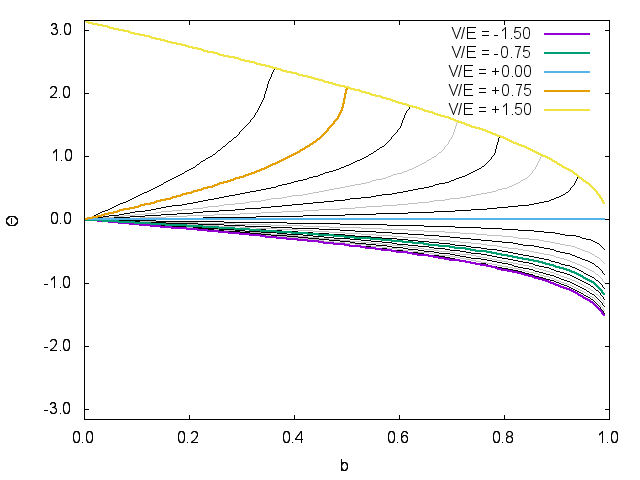
\includegraphics[width=0.8\textwidth]{./plots/01_02}
  \label{fig:analytical}
  \caption{Analytical solutions for varies values of $a$. Gray and black lines indicate intermediate values.}
\end{figure}

\section{Step 3}
In order to numerically integrate our function we use an adaptive Guass-Konrod quadrature (experiments have shown that G7K15 is most performant in this case).
Before integrating, we note that the lower boundaries of the integrals go to infinity from the right. This significantlly hampers the performance of numerical
quadrature methods. In order to reduce this effect we subtract an approximation which is asymptotically equal to the integrand at the lower boundary and analytically solveable.
This makes the total integrand more "polynomial-like" and improves performance. In this case we approximate the function in the square root with a linear expansion around $r_\text{min}$ and
subsequentlly approximate the $1/r$ term in a similar fashion. This leads to an approximation of the form
\begin{align}
  \frac{1}{r^2\sqrt{1-\frac{b^2}{r^2}-\frac{V}{E}}} \approx g(r) = \frac{\left(\alpha+\beta r\right)^2}{\sqrt{\gamma+\lambda r}}
\end{align}
which, while not completely polynominal slightly reduces the functional evaluations needed for similar accuracy and reduces the lower limit on the error. The analyticall integral of this approximation is given by
\begin{align}
  G(r) = \int \frac{\left(\alpha+\beta r\right)^2}{\sqrt{\gamma+\lambda r}} = \frac{2\sqrt{\gamma+\lambda r}\left(15\alpha^2\lambda^2+10\alpha\beta\lambda\left(-2\gamma+r\lambda\right)+\beta^2\left(8\gamma^2-4r\gamma\lambda+3r^2\lambda^2\right)\right)}{15\lambda^3}.
\end{align}
What we then calculate is not $\int_a^bf(r) \d r$ but $\int_a^b f(r)-g(r) \d r + A(r)|_a^b$.

\par For a function of the form of
\begin{align}
  \frac{1}{r^2\sqrt{1-\frac{b^2}{r^2}-a}}
\end{align}
the required constants are given by
\begin{align}
  \alpha &= \frac{\sqrt{1-a}}{b}+\frac{1-a}{b\sqrt{1-a}}\nn
  \beta &= -\frac{1-a}{b^2}\nn
  \gamma &= -2(1-a)\nn
  \lambda &= \frac{2(1-a)^{3/2}}{b}
\end{align}

\par in addition to approximating the integral we will also need to approximate the outermost root of the argument of the square root in order to calculate $r_\text{min}$.
While this can easilly be found to be $-b/\sqrt{1-a}$ in the case of the square potential it requires a numerical approach in the case of the Lennard-Jones potential.
As the point of studying the square potential is to determine the error caused by our method we will also apply the same root-finding method here.
\par we find the root of the argument by first multiplying by the highest inverse power of $r$ ($r^2$ in this case, $r^{12}$ for the Lennard-Jones potential). This introduces the additional root $r=0$ but converts the argument to a polynomial.
We then take this polynomial and find one of its roots using Halley's method, we then use synthetic division to remove this root from the original polynomial and look for another root using the same method. Our stopping criterion is that we must either found all roots, or
Halley's method must have failed to converge in $2^{20}$ steps, which happens when there are no more real roots. The outermost root is then taken to be $r_\text{min}$.

\subsection{results}
In figure \ref{fig:01_03} we have plotted the errors when using various methods of integration. The requested precision for both the roots and the inetgration were set to $10^{-9}$, as we can see the propagated error is still much less than requested error. While the errors
are similar in mean there is a much higher variance the more approximations become involved.

\begin{figure}
  \centering
  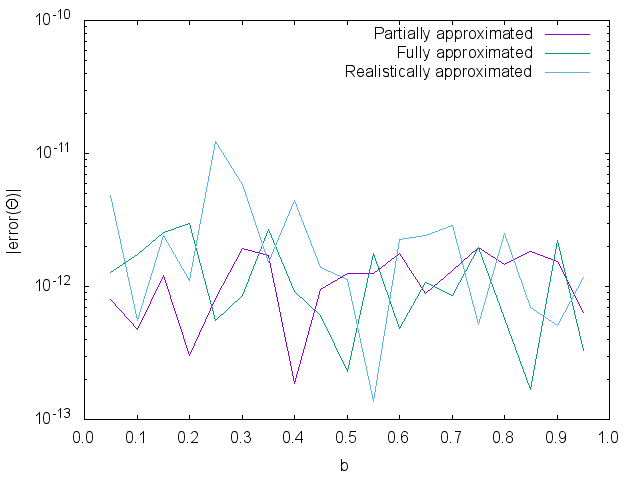
\includegraphics[width=0.8\textwidth]{./plots/01_03}
  \caption{Errors in the deflection function when: integrating only the last term (partial), integrating both terms (full), and integrating only the last term but using root-finding to find the value of $r_\text{min}$ (realistic).}
  \label{fig:01_03}
\end{figure}

\section{Step 4}
We now turn our attention to the Lennard-Jones potential, this potential is given by
\begin{align}
  V = 4\epsilon\left(\left(\frac{\sigma}{r}\right)^{12}-\left(\frac{\sigma}{r}\right)^6\right)
\end{align}
We choose our spatial units in such a way that $\sigma = 1$.
Applying our numerical method as desribed above (analytically integrate the first integral, subtract off the infinity of the second integral, find $r_\text{min}$ using Halley's Method and then integrate using Gauss-Konrod)
produces good results, as shown in figure \ref{fig:01_04}. We see that for certain values of $\epsilon/E$ the deflection function tends to $-\infty$ for certain values of $b$, indicative of orbiting.
\par In figure \ref{fig:01_04b} we have plotted the differential cross section for these energies and positive deflection angles. (negative angles are problematic as the deflection function is not one-to-one here).

\begin{figure}
  \centering
  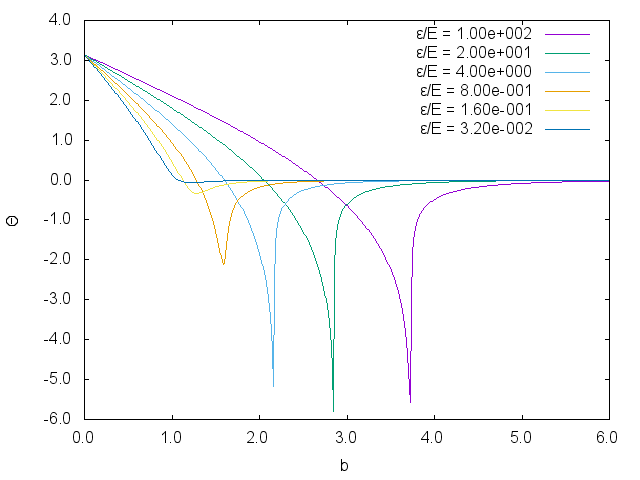
\includegraphics[width=0.8\textwidth]{./plots/01_04}
  \caption{Deflection function for various values of $\epsilon/E$.}
  \label{fig:01_04}
\end{figure}

\begin{figure}
  \centering
  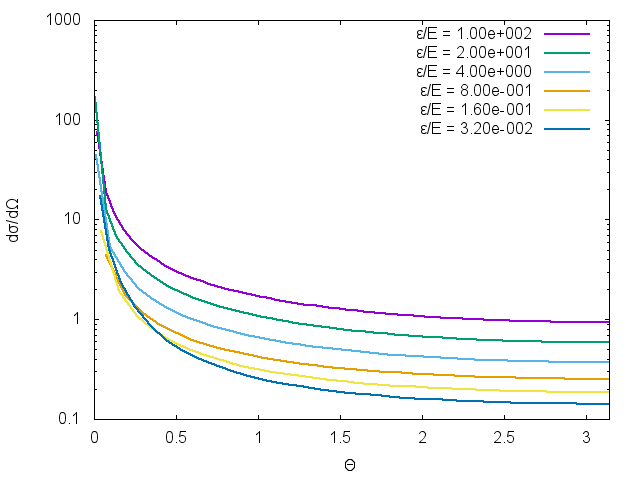
\includegraphics[width=0.8\textwidth]{./plots/01_04b}
  \caption{Differential cross section for various values of $\epsilon/E$.}
  \label{fig:01_04b}
\end{figure}


\section{Step 5}
In order to determine the maximum energy for which the Lennard-Jones potential exhibits
orbiting we define orbiting as having a deflection of less than $-2\pi$. We integrated as before around
points known to exhibit orbiting and gradually reduced the energy by a stepsize $h$ until we no longer observed orbiting,
at which point we returned to the last known orbiting energy and reduced our stepsize, until $h < 10^{-10}$. We also kept track of the location of the minimum for the previous value of the energy so
as to to use this as the upper limit on subsequent searches over $b$ (for the lower limit we used the previous graphs). This greatly speeds up the search. The result found was a limit of $\epsilon/E \approx 1.19317$.
\end{document}
